The objective of this section is to present the main elements of the CPS simulation and synchronization model. However, in order to understand the underlying choices, it is important to clarify its relationship with other elements of the reference architecture presented in Figure~\ref{fig:architecture} and in particular with the components related to the simulation domain. 

In Figure~\ref{fig:architectureSimulation} is an excerpt of the overall reference architecture of FAR-EDGE. 
The simulation domain is envisioned as a layered subsystem of the architecture where the topmost elements are simulation tools and a graphical editor; these rely on the \textit{Open API for Virtualization} to interact with the \textit{Model Repository}, that manages the CPS-based simulation model, and the \textit{Real-to-Digital Synchronization} module that is in charge of supporting the Digital Continuity. 
In particular, the Model Repository manages the virtual shop floor representation, which relies on a shared modeling of core concepts that can be expanded to suit specific purposes; This, in fact, is required to sustain integration of different domains and provision of cloud-based simulation services. 
Lastly, the simulation domain is responsible for developing and openly providing an API for virtualization that, by means of suitable endpoints allows: 
\begin{description}
    \item \textbf{Definition and configuration of simulation scenarios}, that is the platform supports the definition of complete multi-disciplinary CPS models. The API must therefore be able to manipulate the CPS data model to allow the user (or machine constructor) to describe the CPS from different points of view, in order to enable different types of simulations. In addition, the API must support the composition of the CPSs and the subsequent model maintenance.  
    \item \textbf{Execution of simulation scenarios}, including simulation of CPS systems, machine and devices. The platform supports external simulators in leveraging information and digital models of the inputs and outputs of the CPS systems, along with data mining models and statistics (e.g., time series analysis) that are used to describe and determine the outputs of the CPS systems during the simulation.
    \item \textbf{Management of the digital continuity}, that is the process of continuously updating the digital models, including configuration of the Real-to-Digital Synchronization Component and deployment of Synchronization models. 
\end{description}



\begin{figure}
	\centering
	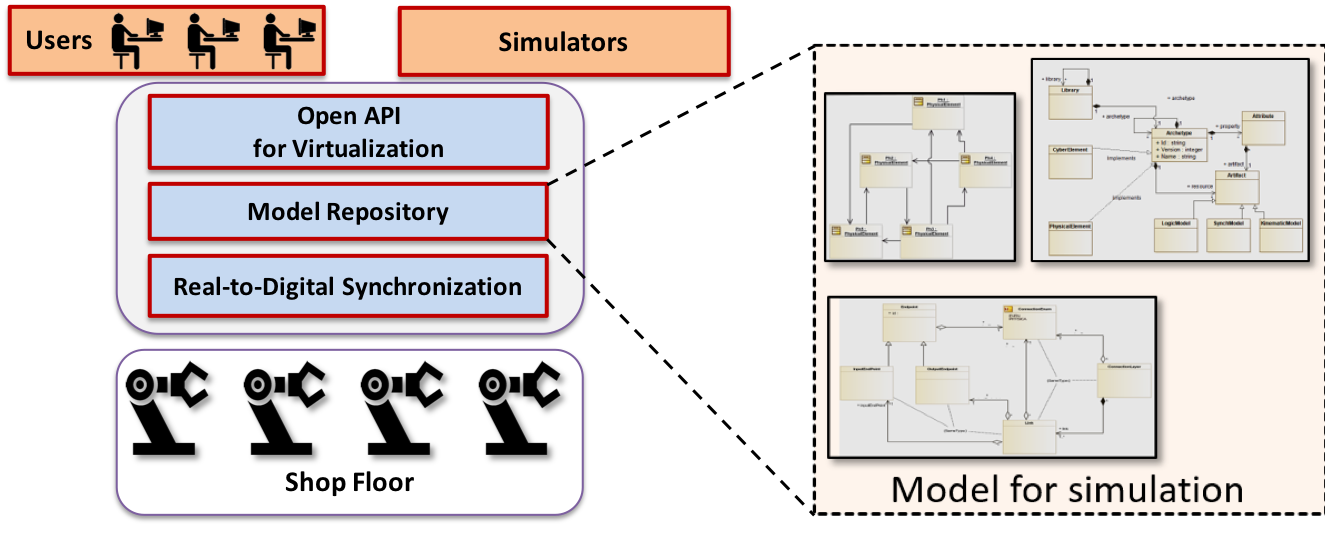
\includegraphics[width=\linewidth]{images/Architecture}
	\caption{Architecture supporting the Digital Continuity}
	\label{fig:architectureSimulation}
\end{figure}





Supporting such ambitious objectives is translated into a set of requirements that data models have to fulfill. 
To this end, our data model needs to be:
\begin{description}
\item[Expressive]- to enable the description of possibly any resource or flow involved in production, logistics and management processes of different industrial domains.
\item[Extensible]- to build, upon a core representation of the factory environment, a growing model ecosystem capable to maintain the digital information available all along the factory life-cycle.
\item[Interoperable]- to provide users with a personalized view and simulation tools that present the virtual environment from their perspective supporting the decision-making processes, activity planning and operation controlling.
\item[Scalable]- that is the ability to function efficiently when the context is changed in size or volume featuring multi-level access features and suitable aggregation patterns.
\item[Modular]- so that it provides representation building blocks that can be rearranged and reconfigured to follow the continuous evolution  of the real factory.
\end{description}


One of the most common features of manufacturing plant design is is to use standardized components (machine tools, robots, etc.) composed in a modular way. 
Through a good organization of modules, in fact, it is possible to speed up engineering as well as the simulation setups, maximizing the reuse of components. 
Similarly, simulation software solutions often provides libraries of models that can be aggregated and extended to assemble full plant layouts.
In this work we aspire to provide the same efficient re-use approach implementing classes to describe resources, called \textit{Archetypes} and \textit{Elements}. %which are instances of such elements and the components of the plant model. 
The Archetype-Element relationship is similar to the one that exists in Object Oriented Programming (OOP)~\cite{wolfgang1994design} between a Class and an Instance (Object) of that class.

Another important requirements is that the resulting data model shall support semantically meaningful collection of relations (referred to as \textit{Layers}). 
We deem particularly important to provide the modelers with a tool to gather links of the same type. 
The idea is to simplify the modeling process by dividing the overall model in several levels. 
By way of example, a first layer may contain the definition of the plant topology with its hierarchies of production resources; the other are graphs that can be used to express relations between resources. 
Logical, electrical, and pneumatic layers are just a few examples of layers.
Finally, in order to achieve flexibility and interoperability the model implements the concept of \textit{artifact}, that is the proposed model support the storage and linking of generic files in the description of the digital twins. 
As a consequence, the modeler can decide to define digital twins using exclusively the syntax and constructs provided by the model (white-box approach), or else use specific and opaque formats whenever (s)he deems it necessary (black-box approach).  
Figure~\ref{fig:layers} illustrates graphically this multi-layer modeling approach. 

\begin{figure}
	\vspace*{-0.5cm}
	\centering
	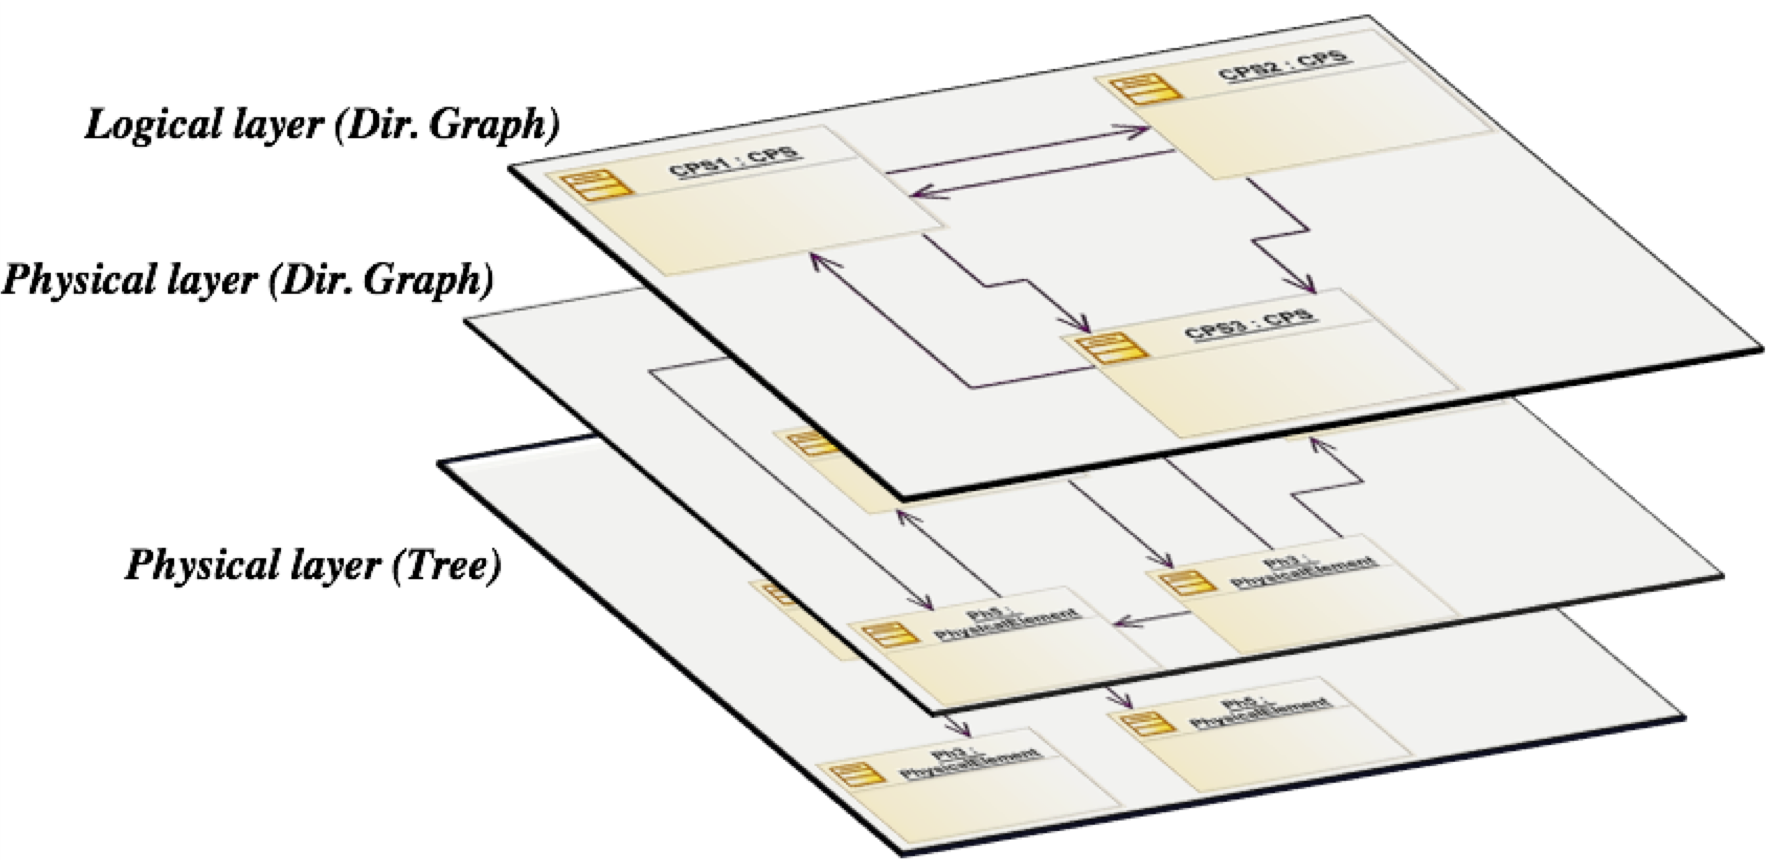
\includegraphics[width=\linewidth]{images/layers2}
	\caption{Modeling using superimposed layers}
	\label{fig:layers}
\end{figure}

This remainder of section documents shortly the data model for simulation and digital continuity, which is organized into 9 areas:

\begin{description}
	\item[\textbf{Core Model}] - documents the core classes used for the definition of  entities and relations used in other sections. The central components of the model are: the \textit{Archetype} and the \textit{Element}. These have a symmetrical structure: both are characterized by one or more roles that identify them semantically, by a unique identifier within the model, by \textit{attributes} (properties used by the modeler to specify Archetypes and Elements), \textit{endpoints} (semantically defined extremes of links connecting Archetypes or Elements) and \textit{artifacts}. 
    \item [\textbf{Archetype Model}] - introduces the concepts of Archetypes as the basis of the model reuse paradigm. Following the OOP paradigm, an Archetype can be seen a moulder that can be used to instantiate \textit{Elements}. The model leaves the user to extend the Archetype concept at will, however, three extensions are provided out-of-the-box, namely, \textit{PhysicalArchetype} (to represent physical resources within a plant), \textit{LogicalArchetype} (to represent the cyber nature of the CPS, used for simulation purposes), \textit{ProductArchetype} (to represent the semi-finished and the final products of the shop) and \textit{TriggerArchetype} (representing an action that can be registered in the platform to be executed in reaction to an event of the shop floor). 
	\item[\textbf{Element Model}] - this model presents the concept of Element as the instantiation of an Archetype according to the OOP.  As said, Archetypes can be defined  as molders used to create specific instances of a certain plant resource. The instances are called Elements. Therefore, Elements are generally created mirroring the structure of their base archetypes, however, unlike  OOP  this is  not  strictly  necessary.  This  means  that  an  element  can  be also defined  as  a  stand-alone  component  or  that  it  is  possible  to add or modify the characteristics inherited from an archetype. 
	\item[\textbf{Connection Model}] - the connection model is devoted to the definition of the links between two model entities.  
To this end, the \textit{Endpoint} class is extended and the concepts of \textit{Link} and \textit{ConnectionLayer} are introduced. 
A Link joins together two instances of the Endpoint class and represents a connection between the elements to which the endpoints belong. 
Links are aggregated in ConnectionLayers and both links and layers can be semantically annotated.

\item[\textbf{Layer Model}] -  extends the concept of layer as a collection of items that can be further specified using attributes. In particular, the user can define collections for Plants (\textit{PlantLayer}), ProductElements (\textit{ProductLayer}), PhysicalElements (\textit{PhysicalLayer}), LogicalElements (\textit{LogicalLayer}) and TriggerElement (\textit{TriggerLayer}).
	\item[\textbf{Attribute Model}] - specifies the concept of property to be used to annotate other elements of the model, namely Library, Archetype, Artifact, and Endpoint. The concept of attribute is further specified as, among the others, \textit{URI}, \textit{Date}, \textit{Number}, \textit{String}, \textit{Composite}, and \textit{Frame}.
	\item[\textbf{Role Model}] - presents a set of classes that defined the concept of Role as semantic description to further specify the constituent elements of the model. The model allows the user to specify an Element/Archetype by assigning a role to it. The \textit{SemanticRole} is the main class of this model. A role has a unique identifier and a name; furthermore, it can contain attributes and be assigned to a library. Finally, a role can refer to other roles to build tree-shaped semantic relationships and to a parent role in order to support the attribute inheritance.
     	\item[\textbf{Plant Model}] - introduces the Plant as an aggregation of layers representing among other aspects its physical and logical nature.  The \textit{Plant} is the main element of this model; it is a specification of the Element class featuring set of resources (physical, logical, and product) as well as their connections. 
Furthermore, a plant also includes several layers. 
Some of them are mandatory and specific as the physical, logical and product layers, which model hierarchies of physical, logical and product entities, respectively.  Other are optional like one or more generic layers, which model graph-shaped relations among the elements of the mandatory layers. Furthermore, Endpoints can be defined to model connections among plants (via Endpoints).
	\item[\textbf{Project Model}] - documents all the classes that represent multi-plant simulation projects, and enable simulation tools to share plant models, scenarios and results.  
\end{description}

This chapter only reports shortly the main elements of the model due to space limitation; a complete and detailed description of the model can be found in~\cite{Ciavotta2018} and \cite{FAR-EDGE41}.

